Commonly, visual models are considered as being simplified versions of complex systems \cite{Bezivin2005} that are obtained by a process of abstraction either from mental concepts or from the properties and features of the sytem itself if it already exists during model creation.
The process of abstraction requires the identification of important properties of the intended system's application and use while omitting properties and features that are considered as being irrelevant for the intended model usage.
In this context, the properties that are captured by the model are requirements on the intended system's application and use.
In most cases, system models are used in contexts where the system itself is still in the process of being developed, i.e., the system is (requirements are) only accessible by means of models during most stages of development.
Therefore, models have an important role in information science \cite{Fetzer20,Thalheim2011} with an image characteristic in the sense that models are (simplified) images of the originals they represent with the purpose to take models as substitutes for their originals within a given temporal and situational context.
The importance of models in information science is addressed by several communities with the object management group (OMG) being one of the largest global initiatives.
Models are the cornerstones of their work where each complex system is rather being designed by means of visual models before being implemented \cite{Janis01}.
This enables a view on problems and their potential solutions before starting with an (extensive) full implementation and therefore, reduces risks. 
At its extreme, the system is developed strictly by modelling and the implementation is (completely) generated from models, i.e., ``the model is the code.'' \cite{Thalheim2011}.

\begin{figure}[!tb]
\begin{center}
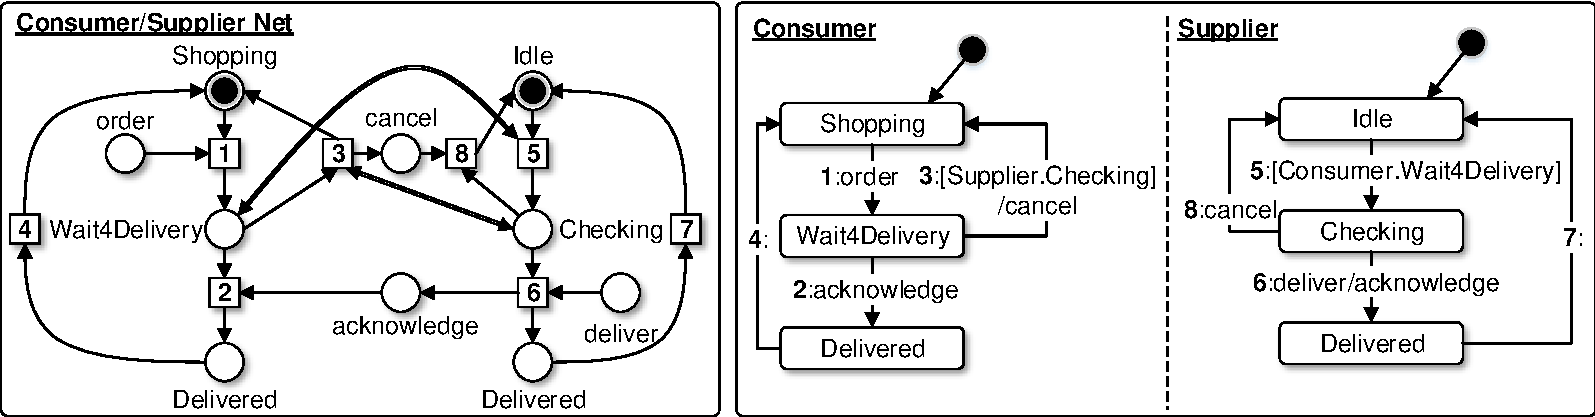
\includegraphics[width=\textwidth]{img/gen_intro/models.pdf}
\end{center}
\caption{Models in Information Science - Place/Transition System (left) \& Statechart (right)}
\label{fig:sec-gen-intro-models:models}
\end{figure}

\begin{figure}[!tb]
\begin{center}
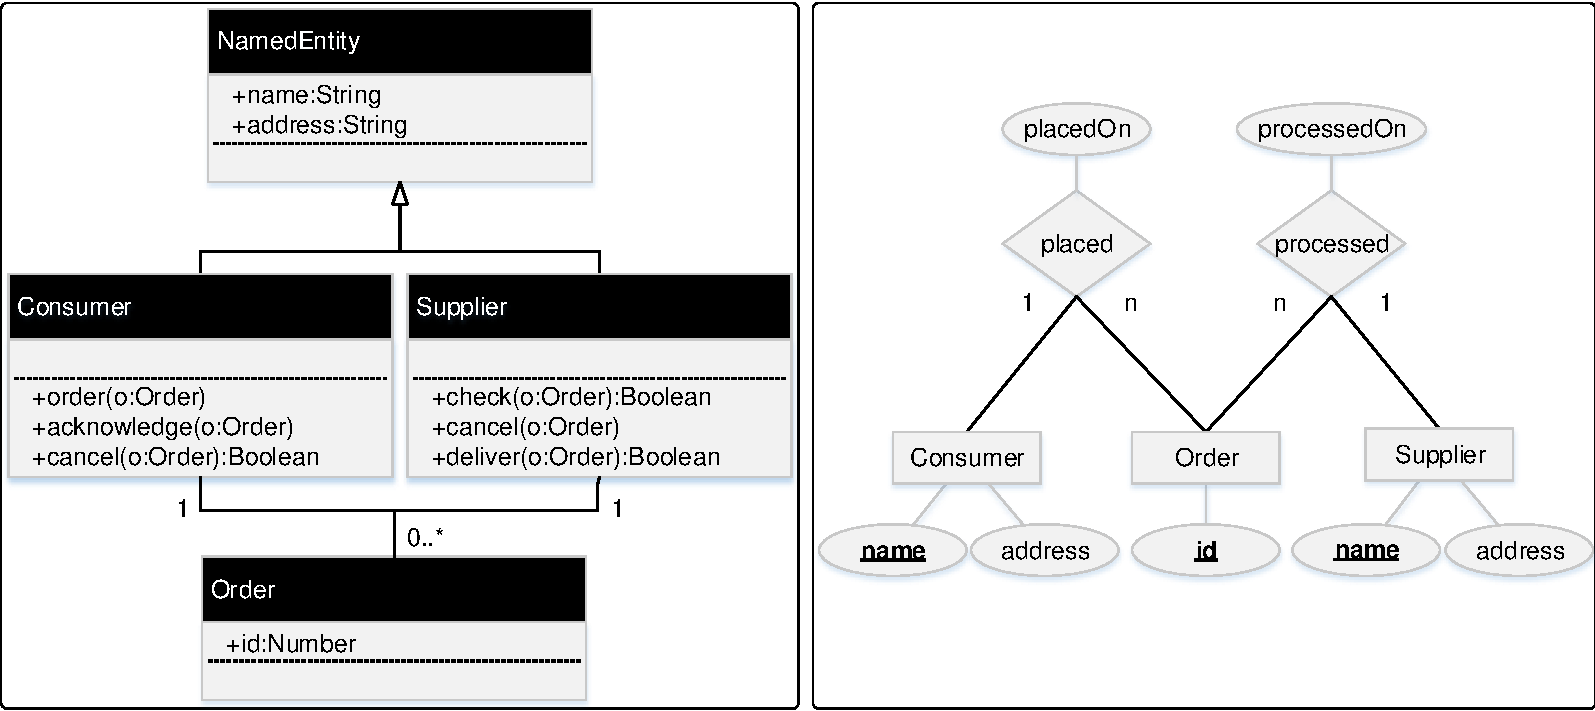
\includegraphics[width=\textwidth]{img/gen_intro/models2.pdf}
\end{center}
\caption{Models in Information Science - UML Class Diagram (left) \& Entity-Relationship Diagram (right)}
\label{fig:sec-gen-intro-models:models2}
\end{figure}

Furthermore it is generally stated that complex systems cannot be comprehended in their entirety, as, the human capacity is limited and therefore, abstractions are necessary that allow us to manage complexity \cite{Quatrani:1998:VMR:275580} by focusing on the relevant details only.
In model-driven software and systems development (MDD), models usually exhibit the following characteristics \cite{Selic:2003:PMD:942589.942714}.
The model must be
{
\renewcommand\labelenumi{(\theenumi)}
\begin{enumerate*}
\item easy to understand for the intended group of model users,
\item accurate, i.e., the model only reflects real properties of the system,
\item predictive, i.e., the model must be a reflection of important, non-obvious properties of a system under development,
\item inexpensive, i.e., the creation and analysis of a model must be cheaper than the implementation of the system and its analysis itself.
\end{enumerate*}
}

Although most models share a common set of properties which make them identifiable as such, Herbert Stachowiak \cite{Stachowiak.1973} and Bernd Mahr \cite{DBLP:journals/sosym/Mahr09,DBLP:journals/eceasst/Mahr10a} each developed a comprehensive theory of model-being.
Instead of identifying an object as a model based on a definition with a fixed set of properties, the model-being of an object is rather the result of a context-specific judgement.
An object $O$ is interpreted as a model $M$ of something $A$ with the purpose for something $B$ and therefore, $O$ carries a cargo (some type of information) from $A$ to $B$.
The model object $O$ is produced based on (a subset of) the properties of original object $A$.
Therefore, these properties must be identifiable in an observation on $O$.
Analogously, purpose $B$ is realised based on (a subset of) the properties of model object $O$.
Therefore, these properties must be identifiable in an observation on the resulting object $B$.
Similarly, \cite{Muller2012} advocates that model-being depends on the existence of a representation relation between model object and its original where a model is considered as the representation of its original.

\cref{fig:sec-gen-intro-models:models,fig:sec-gen-intro-models:models2} depict different types of system models from different perspectives and within different problem domains that are used in MDD \cite{6507223,mdd05,Beydeda2005ModelDriven} for communication between experts of the same domain and across different domains.
\cref{fig:sec-gen-intro-models:models} depicts models of the dynamic behaviour of a given (concurrent) purchase order system that may be used to implement the behaviour in the form of operations in computer programs.
In contrast to \cref{fig:sec-gen-intro-models:models}, \cref{fig:sec-gen-intro-models:models2} depicts models that represent the static organisation of concepts (data) and their interrelationships in the system, i.e., the ontology for the domain of discourse (the purchase order scenario).
These models may be used to implement static aspects of the system, e.g., class definitions in an object-oriented programming language or relational database structures that both may serve as the data basis for the operations in computer programs.

\cref{fig:sec-gen-intro-models:models} (right) illustrates a UML statechart \cite{UML15,Rumbaugh:2004:UML:993859}.
UML statecharts are originated from classical hierarchical Harel statecharts \cite{HAREL1987231,Harel2005} which extend the formalism of finite-state machines \cite{Dathan2015} mostly by hierarchically nested states and orthogonal regions to enhance the readability and scalability of the models.
The statechart consists of (system) states (boxes) and transitions between states (arrows).
Each transition describes some system behaviour by the change from one system state to another state.
Furthermore, the statechart is separated into two orthogonal (concurrently operating) regions as marked by a dashed line.
In each region, the initial state is marked by a black node.
Each transition has an inscription of the form: $[event]['['condition']']['/'action]$ where $[]$ is meant to be optional.
A transition is enabled if the source state of the transition is the current state, the $event$ occured and the $condition$ can be evaluated to true.
If a transition fires, then the current state changes to the target state of the transition and the $action$ is performed.
The following behaviour of a consumer-supplier system is modelled in \cref{fig:sec-gen-intro-models:models} (right):
The consumer and supplier start with \code{Shopping} and \code{Idle}, respectively.
After \code{Shopping}, the consumer may decide to \code{order} and consequently, waits for delivery afterwards (state \code{Wait4Delivery}).
If the consumer is waiting for delivery, the supplier immediately pass over to \code{Checking} the order.
As long as the supplier is \code{Checking} and the consumer is waiting, the consumer may \code{cancel} the order at any time which directly causes a cancellation on the supplier side.
After cancellation both sides return to their initial states.
After \code{Checking}, the supplier may decide to deliver the ordered items while asking the consumer to \code{acknowledge} the receipt at the same time.
Subsequently, the consumer \code{acknowledge}s, both transition into state \code{Delivered} and may return to their initial states at any time.
 
\cref{fig:sec-gen-intro-models:models} (left) depicts a Petri net, more precisely a place/transition net with initial marking \cite{NIELSEN19923,Reisig:1985:PNI:3405}, which captures the same dynamic behaviour from \cref{fig:sec-gen-intro-models:models} (right).
The marking is given by a (black) token distribution which defines the system state.
By firing an enabled transition (boxes) the state can be changed.
A transition is enabled, if each input place (circles with outgoing edges to the corresponding transition) contains a token.
When a transition is fired, all tokens from the input places are removed and for each output place (circles with incoming edges from the corresponding transition) a token is added.
Therefore, for each transition in \cref{fig:sec-gen-intro-models:models} (right) there is a transition defined in \cref{fig:sec-gen-intro-models:models} (left) and the initial states (each state and event) in the statechart are (is) modelled by an initial marking (a place) in the net.

While the statechart delivers a readable model of the behaviour, the Petri net may be used for formal analysis of the behaviour as supported by a variety of existing tools.

\cref{fig:sec-gen-intro-models:models2} (left) presents a UML class diagram \cite{UML15,Rumbaugh:2004:UML:993859}.
The diagram designates classes \code{Consumer}, \code{Supplier} and \code{Order} as central concepts of the system.
\code{Consumer}s and \code{Supplier}s are named entities (cf. inheritance relationship with class \code{NamedEntity}) and therefore, they have a \code{name} and \code{address} both of type \code{String}.
Furthermore, a \code{Consumer} has the following operations (possible behaviour):
A \code{Consumer} may:
\begin{enumerate*}
\item place an \code{Order} \code{o},
\item \code{acknowledge} the receipt of an \code{Order} \code{o}, or
\item \code{cancel} an \code{Order} \code{o} with \code{Boolean} return value. By \cref{fig:sec-gen-intro-models:models}, a cancellation is only possible if the \code{Supplier} is checking the order as indicated by a \code{Boolean} return value which returns \code{true} in case of success and otherwise \code{false}.
\end{enumerate*}
Similarly, a \code{Supplier} may:
\begin{enumerate*}
\item \code{check} an \code{Order} \code{o},
\item \code{cancel} an \code{Order} \code{o}, or
\item \code{deliver} an \code{Order} \code{o}.
\end{enumerate*}
Furthermore by the interrelationships as given in the diagram:
\begin{enumerate*}
\item Each \code{Consumer} may have placed an arbitrary number of \code{Order}s, each \code{Order} identified by an \code{id},
\item each \code{Supplier} may have processed an arbitrary number of \code{Order}s, and
\item each \code{Order} was placed (processed) by exactly one \code{Consumer} (\code{Supplier}).
\end{enumerate*}

\cref{fig:sec-gen-intro-models:models2} (right) presents an entity-relationship diagram containing the same concepts and interrelationships from the class diagram.
However, note that the operations (suggestions of possible behaviour) of the entities are missing, the interrelationships \code{placed} and \code{processed} become explicit figures with additional attributes \code{placedOn} and \code{processedOn} instead of simple arrows and attributes \code{name} and \code{id} are particularly marked as unique instance identifiers (primary keys).

Therefore, the class diagram is rather used to generate the base frame of a program in an object-oriented programming language while the entity-relationship diagram is used to create the structure of a relational database that may be used by the program.